\documentclass{article}

\usepackage{graphicx}
\usepackage{xcolor}
\usepackage{hyperref}
\usepackage{amsmath}

\title{Quantum computing TP\\ Phase estimation for quantum chemistry}


\author{\textbf{Supervisor:} Bertrand Marchand}


\begin{document}
\maketitle
\begin{abstract}
You need to fill up some notebook cells with your implementation according to the questions.
\textbf{Send the completed notebook file by next Thursday, Janurary 14 2021}, by mail to bertrand.marchand7@gmail.com. 
It will be corrected and graded.
\end{abstract}

\section{Quantum Programming Basics}

\paragraph{Question 1} Implement the following circuit, simulate it for $\theta=0.3$, and print all states along with their amplitudes and probabilities.

\begin{center}
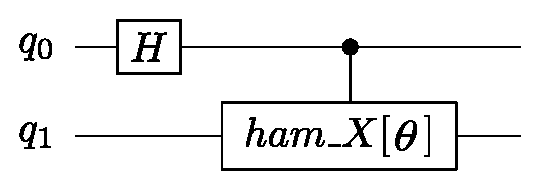
\includegraphics[width=.7\textwidth]{qat2pdf_llce_fji_circ.pdf}
\end{center}

Where $ham\_X(\theta) = e^{-i\theta X}$ with $X=\begin{pmatrix}0 & 1 \\ 1 & 0\end{pmatrix}$

\paragraph{Hint} Define $ham\_X$ as an ``AbstractGate'', then apply it using ``.ctrl()'' to get a controlled version, as suggested in 
the ``minimal notebook''. Don't hesitate to also refer to the slides that were sent to you, for instance for the definition of what
a controlled gate is (slide 2).

\section{Iterative quantum phase estimation, reproducing results from \textcolor{blue}{\cite{o2016scalable}}}

\subsection{Hamiltonian simulation}

The Hamiltonians whose ground state energy we are trying to compute are of the form: 
$$H(R) = g_{0}I+g_{1}ZI+g_{2}IZ+g_{3}ZZ+g_{4}YY+g_{5}XX $$

Because we use \textbf{Trotterization}, we will only have
to implement the unitary evolutions generated by each of the
individual terms: $e^{-iXXdt}$, $e^{-iZIdt}$, 
$e^{-iIZdt}$, $e^{-iZZdt}$, $e^{-iYYdt}$ and $e^{-iXXdt}$.

\paragraph{}
We could implement them using Abstract gates and a numerical
computation of the matrix exponential. But the computation of the
matrix exponential does not scale well with the number of qubits, 
and thus this method cannot be used in the ``general case'', when
working with a large molecule.

What we will do therefore instead is find small parametrized circuits 
implementing each of the unitary evolutions. The small circuits
may only use ``usual gates'', such as CNOTs and single-qubit Pauli
rotations, that are already pre-implemented in PyAQASM/myqlm.
We will then use \textbf{QRoutines} to paste these circuits into
the final algorithm. Such a method does yield circuits of polynomial
size for arbitrary Pauli products over $n$ qubits.

\paragraph{}
\textbf{Example}:
You can check that: $Z\otimes Z = CNOT_{0\rightarrow 1} \cdot I\otimes Z \cdot CNOT_{0\rightarrow 1} $\\~\\
with $CNOT_{0\rightarrow 1}=\begin{pmatrix} 1 & 0 & 0 & 0 \\ 0 & 1 & 0 & 0 \\ 0 & 0 & 0 & 1 \\ 0 & 0 & 1 & 0 \end{pmatrix}$, $\otimes$
the Kronecker product and $\cdot$ the standard matrix product.\\~\\
It allows us to write: 
\begin{align*}
e^{-iZZdt} &= e^{-i(CNOT_{0\rightarrow 1})\cdot (IZ)\cdot (CNOT_{0\rightarrow 1})dt}\\ 
           &= CNOT_{0\rightarrow 1}\cdot e^{-iIZdt} CNOT_{0\rightarrow 1}\\
           &= CNOT_{0\rightarrow 1}\cdot \left(I\otimes e^{-iZdt}\right)\cdot CNOT_{0\rightarrow 1}
\end{align*}
i.e:
\begin{center}
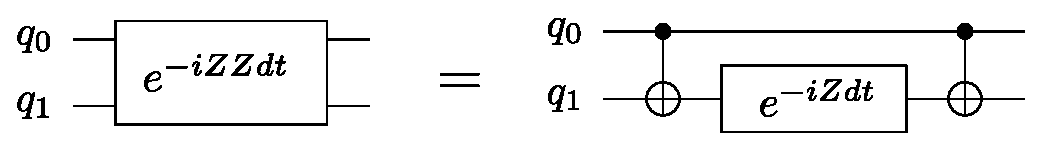
\includegraphics[width=.5\textwidth]{zz_rz.eps}
\end{center}


where $e^{-iZdt} = \begin{pmatrix} e^{-idt} & 0 \\ 0 & e^{idt} \end{pmatrix} = RZ(2*dt)$.

\paragraph{} $RZ$ is a ``standard gate'', pre-implemented in PyAQASM, defined as $RZ(\theta)=e^{-i\frac{\theta Z}{2}}$.
Likewise, $RX(\theta) = e^{-i\frac{\theta X}{2}}$ and 
$RY(\theta)=e^{-i\frac{\theta Y}{2}}$ are pre-implemented. You can look at their precise definitions
\textcolor{blue}{\href{https://myqlm.github.io/aqasm.html\#aqasm}{here}}.

\paragraph{Question 2} Following the example above, which is already implemented in the notebook, and knowing in addition that:
$$ X\otimes X = CNOT_{0\rightarrow 1} \cdot X\otimes I \cdot 
CNOT_{0\rightarrow 1}  $$
$$ SXS^{\dagger} = Y $$ with $S=\begin{pmatrix}1 & 0 \\ 0 & i \end{pmatrix}$ \\and 
$$ Y\otimes X = CNOT_{0\rightarrow 1} \cdot Y\otimes I \cdot 
CNOT_{0\rightarrow 1} $$
write down the QRoutines carrying out each of the required 
Hamiltonian simulations, by filling the templates already written
in the notebook. 

\subsection{Iterative Phase estimation}

\subsubsection{Trotterization}

\textbf{Question 3} Write a function taking as input hamiltonian
coefficients, an interval of time $dt$,  and a Trotter number $p$, 
and returning a Qroutine which implements the corresponding
Trotterized implementation of the Hamiltonian.

We recall that Trotterization consists in approximating $e^{-idt\left(\sum_{l}c_{l}H_{l}\right)}$ as
$\left(\prod_{l}e^{-i\frac{dt c_{l} H_{l}}{p}}\right)^{p}$. Therefore, your Qroutine should make use of
the other Qroutines you implemented in Question 2. As for the coefficients weighting the influence
of each individual terms, they are available in the list of dictionaries loaded at the beginning
of the notebook, from {\fontfamily{lmr}\selectfont hamiltonian\_data.json}. As specified in the notebook,
your function should also take an "energy shift" as input parameter. It consists in adding a $+shift\cdot I$
term to your Hamiltonian. We will use it to ensure the energies we compute are $>0$. Take a look at the 
slides (slide 10) for more explanations.

To be more explicit, the QRoutine should implement:
$$ dt, p \rightarrow \left[e^{-i\frac{g_{0}dt}{p}I}e^{-i\frac{g_{1}dt}{p}ZI}e^{-i\frac{g_{2}dt}{p}IZ}e^{-i\frac{g_{3}dt}{p}ZZ}e^{-i\frac{g_{4}dt}{p}YY}e^{-i\frac{g_{5}dt}{p}XX}\right]^{p} $$

We recall that: $H=g_{0}I + g_{1}ZI + g_{2}IZ + g_{3}ZZ + g_{4}YY + g_{5}XX$

\subsubsection{Iterative Phase estimation}

\begin{figure}
\centering
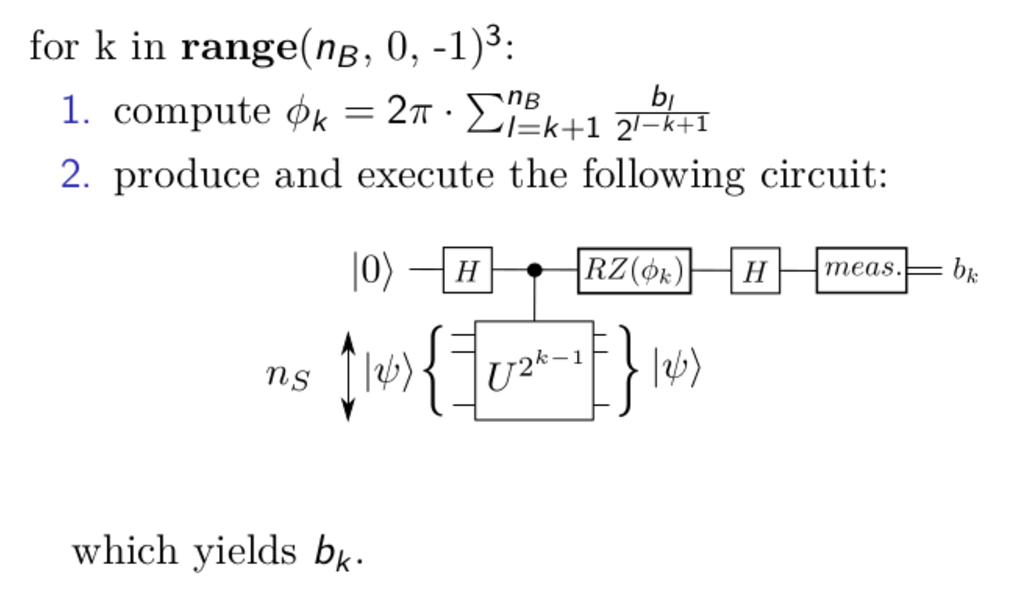
\includegraphics[width=.6\textwidth]{pseudo_code.eps}
\caption{The pseudocode and circuit to implement at \textbf{Question 4}}
\label{pseudocode}
\end{figure}

\paragraph{Question 4} Implement iterative phase estimation following the template provided in the notebook, 
the definitions given in the slides (slide 6) and Figure~\ref{pseudocode}.

In a few words, you need to loop over $k=n_{B},...,1$ in that order, and for each of these values:
\begin{itemize}
\item Produce the circuit displayed on the slides (slide 6) and Figure~\ref{pseudocode}. 
Depending on the value of the ``trotterization'' Boolean
flag, the Hamiltonian simulation can either be the ideal ``cheat mode'' version that exponentiates the Hamiltonian,
or the Trotterized version you implemented. In place of ``$|\psi\rangle$'', the ground state of the Hamiltonian,
we will use a simple ansatz, the Hartree-Fock approximation to our problem: $|10\rangle=(X\otimes I)|00\rangle$, as suggested in
\textcolor{blue}{\cite{o2016scalable}}, and explained in the slides (slide 10).
\item simulate the circuit, specifying at job creation that you are interested in the first qubit only, and 
select the most probable result\footnote{Of course in a real setting we would have to run the circuit many times
to estimate the probabilities, here, we compute them numerically.}.
\end{itemize}

\subsection{final plots}

\paragraph{Question 5} The cells actually computing the curves are already written, for the most part. The only
thing you need to fill is the conversion of phases back to energies. Put your implementation where indicated and produce the plots.
The ``ideal'' result should be a smooth $H_{2}$ dissociation curve, while the Trotterized version should be more ``wiggly'',
the curve with $p=10$ being a closer approximation to the ideal curve, as expected.

\appendix
\section{tensor products, matrix exponential and Pauli matrices}

\subsection{Pauli matrices}

$$ X = \begin{pmatrix} 0 & 1 \\ 1 & 0 \end{pmatrix} $$

$$ Y = \begin{pmatrix} 0 & -i \\ i & 0 \end{pmatrix} $$

$$ Z = \begin{pmatrix} 1 & 0 \\ 0 & -1 \end{pmatrix} $$

\subsection{tensor products}

$$ (A\otimes B)\cdot (C\otimes D) = AC\otimes BD $$

$$ I\otimes A^{\dagger} = I^{\dagger}\otimes A^{\dagger} = 
(A\otimes I)^{\dagger}   $$

with $I$ the plain identity matrix.
\subsection{matrix exponential}

\begin{align*}
e^{U^{\dagger}AU} &= \sum_{k=0}^{+\infty} \frac{(U^{\dagger}AU)^{k}}{k!} \\ 
&= \sum_{k=0}^{+\infty} \frac{U^{\dagger}A^{k}U}{k!} \\ 
&= U^{\dagger}\sum_{k=0}^{+\infty} \frac{A^{k}}{k!}U \\ 
&= U^{\dagger}e^{A}U \\ 
\end{align*}

This is what happens with $CNOT_{0\rightarrow 1}$
in the example that is given.

\bibliography{biblio}
\bibliographystyle{unsrt}
\end{document}
